\documentclass[a4paper, 12pt]{extarticle}

%%% Includes 
\usepackage[utf8]{inputenc} % UTF-8 encode 
\usepackage[english, russian]{babel}
\usepackage{geometry} % adjust page layout 
\usepackage{graphicx} 
\usepackage{hyperref} 
\usepackage{amsmath} % math formulas 
\usepackage{setspace} % for set line spacing 
\usepackage{indentfirst} % indent on a first line after the paragraph 
% \usepackage{pgfplots} % for plots 
\usepackage{listings} % for code listings 
\usepackage{xcolor} % colors (used for listings)
\usepackage{sourcecodepro} % for another monospaced font 
\usepackage{cmap} % for correct search in pdf
\usepackage{placeins} % for \FloatBarrier


%%% Debug
% \usepackage{showframe} % frame borders for demonstration 


%%% Custom commands
% commands for unnumbered sections
\newcommand{\usection}[1]{\section*{#1} \addcontentsline{toc}{section}{\protect\numberline{}#1}}
\newcommand{\usubsection}[1]{\subsection*{#1} \addcontentsline{toc}{subsection}{\protect\numberline{}#1}}
\newcommand{\usubsubsection}[1]{\subsubsection*{#1} \addcontentsline{toc}{subsubsection}{\protect\numberline{}#1}}


% Redefinition of section and subsection numbering style (with dot at the end)
\def\thesection{\arabic{section}.}
\def\thesubsection{\arabic{section}.\arabic{subsection}.}
\def\thesubsubsection{\arabic{section}.\arabic{subsection}.\arabic{subsubsection}.}



%%% Settings for links 
\hypersetup{
    colorlinks,
    citecolor=black,
    filecolor=black,
    linkcolor=black,
    urlcolor=black
}



%%% Layout
\geometry{
	left=17mm, % left margin
	top=17mm, % top margin
	right=17mm, % right margin
	bottom=20mm, % bottom margin
	marginparsep=0mm, % space between text and margin notes
	marginparwidth=0mm, % width of margin notes
	headheight=8mm, % height of the header
	headsep=5mm, % space between header and text
}


\linespread{1.5} % line spacing
\setlength{\parskip}{\baselineskip}  % Add space between paragraphs


% overfull hbox settings
\tolerance 5000 % default 200, max 10000, 
\hbadness 3000 % default 1000, max 10000, warning threshold for underfull hbox
\emergencystretch 0pt  % default 0pt, how much the lines can stretch for the sake of good line breaks
\hfuzz 0.4pt % ignore overfull box less than 
\widowpenalty=10000 % no lines at the start of the page
\vfuzz \hfuzz % don't care about underfull vbox if overfull is acceptable
\raggedbottom % if the page is not filled, align the content to the bottom


%%% Redefinition of table of contents command to get centered heading
\makeatletter
\renewcommand\tableofcontents{ 
  \begin{singlespace}
    \null\hfill\textbf{\Large\contentsname}\hfill\null\par
    \@mkboth{\MakeUppercase\contentsname}{\MakeUppercase\contentsname}%
    \@starttoc{toc}
  \end{singlespace}
}
\makeatother


%%% Listings settings
\definecolor{codegreen}{rgb}{0, 0.6, 0}
\definecolor{codegray}{rgb}{0.5, 0.5, 0.5}
\definecolor{codepurple}{rgb}{0.58, 0, 0.82}
\definecolor{backcolour_gray}{rgb}{0.98, 0.98, 0.98}

\lstdefinestyle{python_white}{
  language=Python,
  backgroundcolor=\color{backcolour_gray},   
  commentstyle=\color{codegreen},
  keywordstyle=\color{blue},
  numberstyle=\tiny\color{codegray},
  stringstyle=\color{codepurple},
  basicstyle=\ttfamily\small\singlespacing,
  breakatwhitespace=true,         
  breaklines=true,                 
  captionpos=b, % t/b                  
  keepspaces=true,                 
  numbers=none, % none/left/rigth                    
  numbersep=5pt,                  
  showspaces=false,                
  showstringspaces=false,
  showtabs=false,                  
  tabsize=2,
  frame=single, % none/leftline/topline/bottomline/lines/single/shadowbox
  rulecolor=\color{gray}, % frame color 
}

\lstset{style=python_white} % set default listings style


% For title page
\def\name{Отчет по лабораторной работе №4} 
\def\subname{Сегментация изображений}
\def\madeby{Александр Иванов, Ф ТЕХ.ЗРЕНИЕ 1.1 \\ Ани Аракелян, ТЕХ.ЗРЕНИЕ 1.1\\ Никита Братушка, ТЕХ.ЗРЕНИЕ 1.3}
\def\teacher{Шаветов С. В.}

\begin{document}

% Title page 
\begin{titlepage}

\thispagestyle{empty}

\title{


\includegraphics[width=4cm]{media/ITMO_logo.png} 

\vspace{1em}
НИУ ИТМО 
\vspace{4em}

\begin{center}
\large\textsc{\textbf{\name}}

\vspace{1em}
``\subname'' 

\end{center}

\vspace{3em}

\begin{flushright}
\normalsize{ 
Выполнили: \\ \textbf{\madeby} 

Преподаватель: \\ \textbf{\teacher} 
}
\end{flushright}	

\vfill

\begin{center}
\small{Санкт-Петербург, \the\year}
\end{center}
}


\author{}
\date{}
\maketitle
\thispagestyle{empty}
\end{titlepage} % Title page

\addtocounter{page}{1} % Inc counter to start from 2 
\tableofcontents % Table of contents
\pagebreak

\section{Вступление}

Продолжая тему печального состояния молодежи, возьмем для работы следующее фото (см. рисунок \ref{img:source}):
\begin{figure}[ht!]
    \centering
    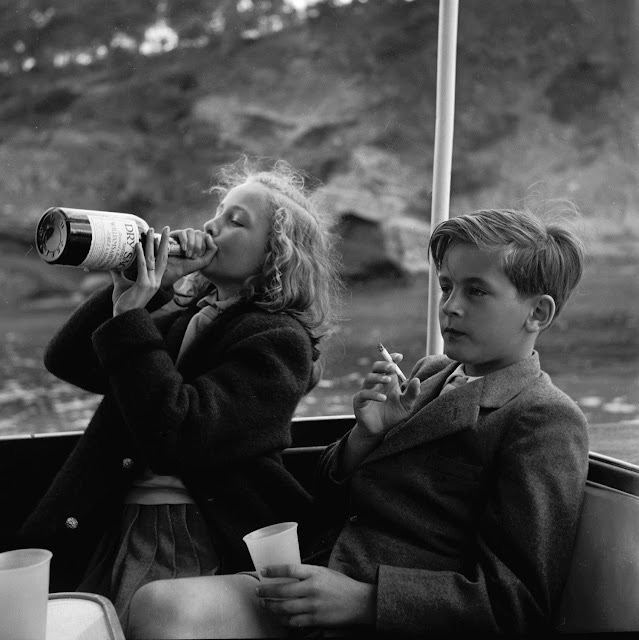
\includegraphics[width=0.8\textwidth]{../image.png}
    \caption{Исходная фотография}
    \label{img:source}
\end{figure}

Опустив лекцию о моральном упадке, перейдем к технической части. 


\FloatBarrier

\section{Бинаризация изображений}

Бинаризация изображения выполняется по следующему алгоритму:
\begin{equation}
    I_{new}(x, y) = \begin{cases}
        0, & I(x, y) \le t,\\
        1, & I(x, y) > t,
    \end{cases}
\end{equation}
где $t$ -- порог бинаризации. 

Или, в случае двойного порога: 
\begin{equation}
    I_{new}(x, y) = \begin{cases}
        0, & I(x, y) \le t_1,\\
        1, & t_1 < I(x, y) \le t_2, \\
        0, & I(x, y) > t_2
     \end{cases}
\end{equation}
где $t_1$, $t_2$ -- верхний и нижний порог бинаризации соответственно. 


\FloatBarrier
\subsection{Бинаризация по среднему значению}
В данном случае, в качестве порога выберем средние значение яркости пикселей, вычисляемое по формуле
\begin{equation}
    t = \frac{I_{max} - I_{min}}{2}
\end{equation}
где $I_{max}$ -- максимальное значение яркости пикселей, $I_{min}$ -- минимальное значение яркости пикселей.

Полученное в результате бинаризации изображение представлено на рисунках \ref{img:binarization_mean} и~\ref{img:binarization_mean_inv}. Значение порога бинаризации при этом оказалось равным 127.
\begin{figure}[ht!]
    \centering
    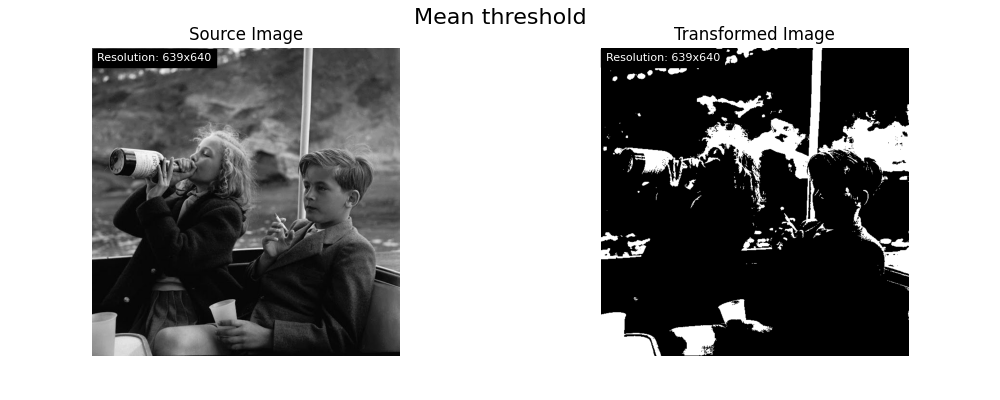
\includegraphics[width=\textwidth]{../results/Mean threshold.png}
    \caption{Результат бинаризации по среднему значению}
    \label{img:binarization_mean}
\end{figure}

\begin{figure}[ht!]
    \centering
    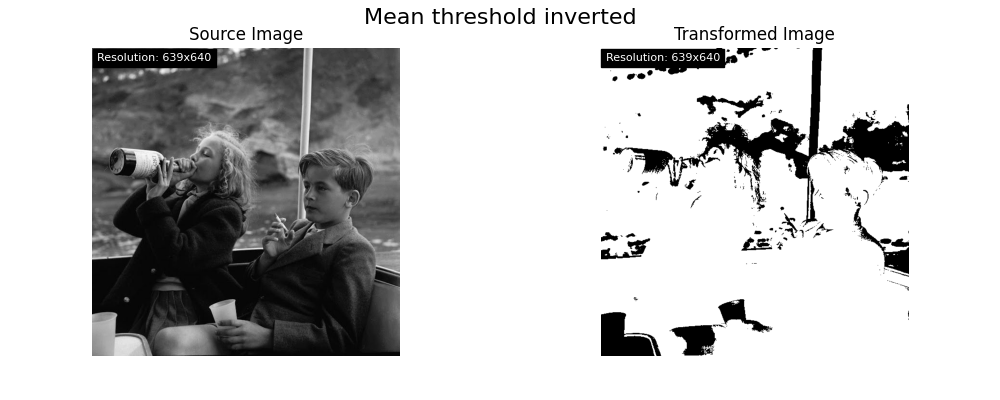
\includegraphics[width=\textwidth]{../results/Mean threshold inverted.png}
    \caption{Результат бинаризации по среднему значению (инвертированная)}
    \label{img:binarization_mean_inv}
\end{figure}

Видим, что, как и ожидалось, в случае с бинаризацией по нижнему порогу, все пиксели темнее среднего значения стали черными, а светлее -- белыми. В случае бинаризации по верхнему порогу, наоборот, все пиксели светлее среднего значения стали черными, а темнее -- белыми.


\FloatBarrier
\subsection{Бинаризация по модулю градиента}
В данном случае значение порога бинаризации $t$ выбирается по следующей формуле:
\begin{equation}
    t = \frac{\sum_{x = 0}^{X - 1}\sum_{y = 0}^{Y - 1}I(x, y)G(x, y)}{\sum_{x = 0}^{X - 1}\sum_{y = 0}^{Y - 1}G(x, y)}
\end{equation} 
где $G(x, y)$ -- модуль градиента изображения, вычисляемый по формуле: 
\begin{equation}
    G(x, y) = \max{|I(x + 1, y) - I(x - 1, y)|, |I(x, y + 1) - I(x, y - 1)|}
\end{equation}
Исходный код для вычисления порога бинаризации на основе градиента представлен в листинге \ref{lst:calc_gradient_threshold}.

Полученное в результате бинаризации изображение представлено на рисунке \ref{img:binarization_gradient} и~\ref{img:binarization_gradient_inv}. Значение порога бинаризации при этом оказалось равным 196.
\begin{figure}[ht!]
    \centering
    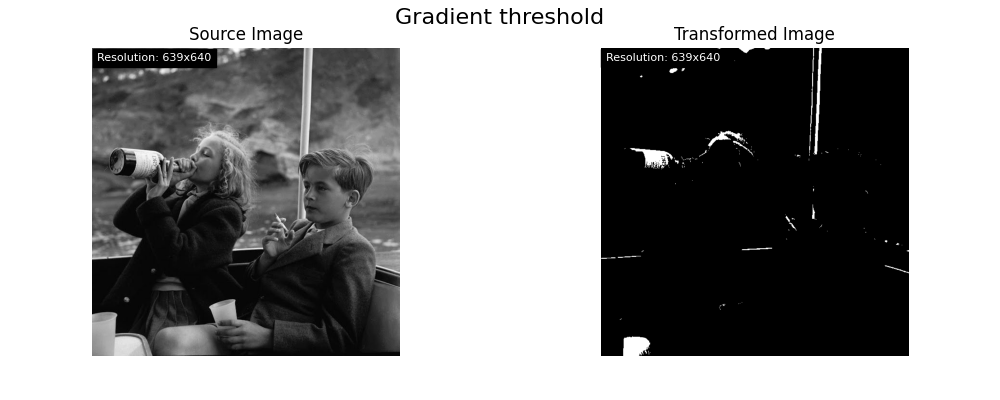
\includegraphics[width=\textwidth]{../results/Gradient threshold.png}
    \caption{Результат бинаризации по модулю градиента}
    \label{img:binarization_gradient}
\end{figure}

\begin{figure}[ht!]
    \centering
    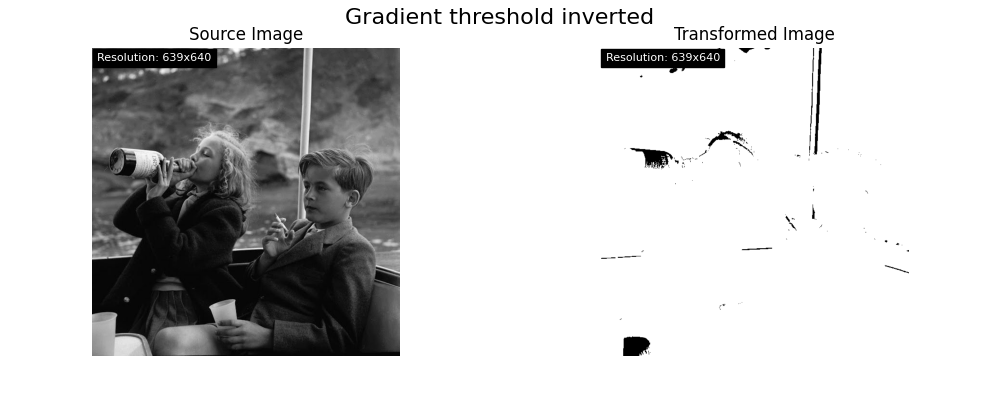
\includegraphics[width=\textwidth]{../results/Gradient threshold inverted.png}
    \caption{Результат бинаризации по модулю градиента (инвертированная)}
    \label{img:binarization_gradient_inv}
\end{figure}

Видим, что при увеличении значения порога бинаризации, увеличивается количество черных пикселей на изображении.

Метод вычисления порога бинаризации на основе градиента показал себя на данном изображении не лучшим образом. Оно практически все стало черным. 

\FloatBarrier
\subsection{Бинаризация по методу Отсу}

В методе Отсу порог бинаризации выбирается таким образом, чтобы минимизировать внутриклассовую дисперсию и максимизировать межклассовую дисперсию.
В Python есть реализация метода Отсу в библиотеке OpenCV. Полученное в результате бинаризации изображение представлено на рисунке \ref{img:otsu_threshold} и~\ref{img:otsu_threshold_inv}.

В данном случае значение порога бинаризации $t$ оказалось равным 78.
\begin{figure}[ht!]
    \centering
    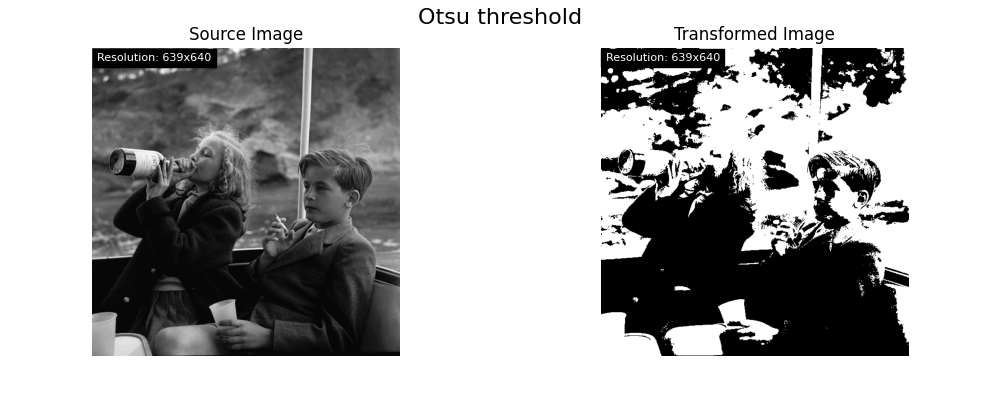
\includegraphics[width=\textwidth]{../results/Otsu threshold.png}
    \caption{Результат бинаризации по модулю Отсу}
    \label{img:otsu_threshold}
\end{figure}

\begin{figure}[ht!]
    \centering
    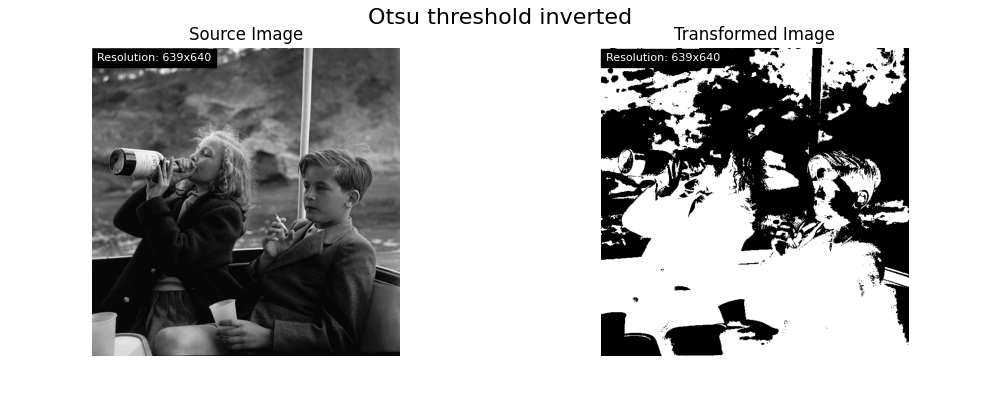
\includegraphics[width=\textwidth]{../results/Otsu threshold inverted.png}
    \caption{Результат бинаризации по модулю Отсу (инвертированная)}
    \label{img:otsu_threshold_inv}
\end{figure}

Бинаризация на основе алгоритма Отсу хороша сработала в данном случае. На изображении, хоть оно и является черно-белым, хорошо различимы объекты.

\FloatBarrier
\subsection{Адаптивная бинаризации}

Адаптивная бинаризация позволяет учитывать различные особенности изображения, такие как освещенность, контрастность и т.д. В данной работе рассмотрены два метода адаптивной бинаризации: на основе среднего и на основе функции Гаусса.

\subsubsection{Анаптивная бинаризация на основе среднего}

\begin{figure}[ht!]
    \centering
    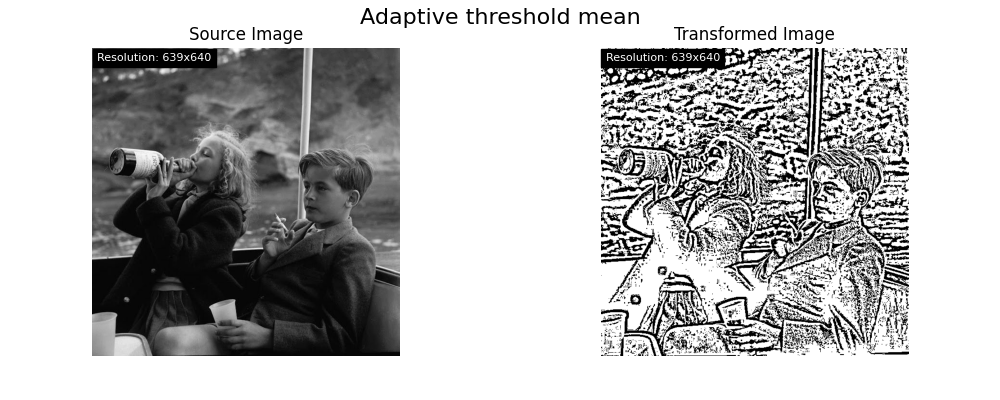
\includegraphics[width=\textwidth]{../results/Adaptive threshold mean.png}
    \caption{Результат адаптивной бинаризации на основе среднего}
    \label{img:adaptive_mean}
\end{figure}

\begin{figure}[ht!]
    \centering
    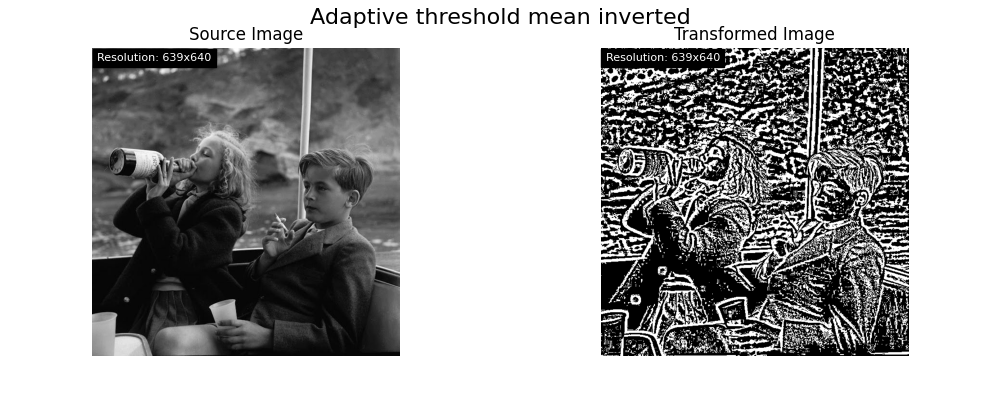
\includegraphics[width=\textwidth]{../results/Adaptive threshold mean inverted.png}
    \caption{Результат адаптивной бинаризации на основе среднего (инвертированная)}
    \label{img:adaptive_mean_inv}
\end{figure}

Этот метод бинаризации отличается от всех ранее рассмотренных. Субъективно, он больше похож на алгоритм выделения контуров, чем на бинаризацию. 
\FloatBarrier
\subsubsection{Анаптивная бинаризация на Функции Гаусса}

\begin{figure}[ht!]
    \centering
    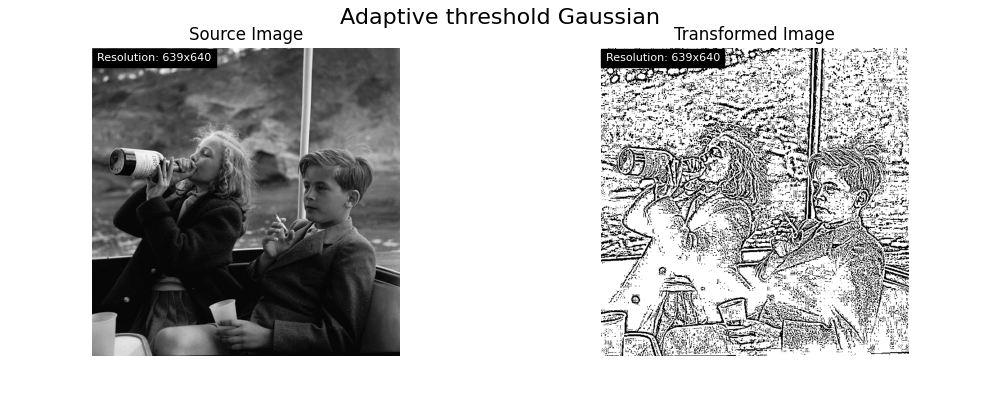
\includegraphics[width=\textwidth]{../results/Adaptive threshold Gaussian.png}
    \caption{Результат адаптивной бинаризации на основе функции Гаусса}
    \label{img:adaptive_gaussian}
\end{figure}

\FloatBarrier
\begin{figure}[ht!]
    \centering
    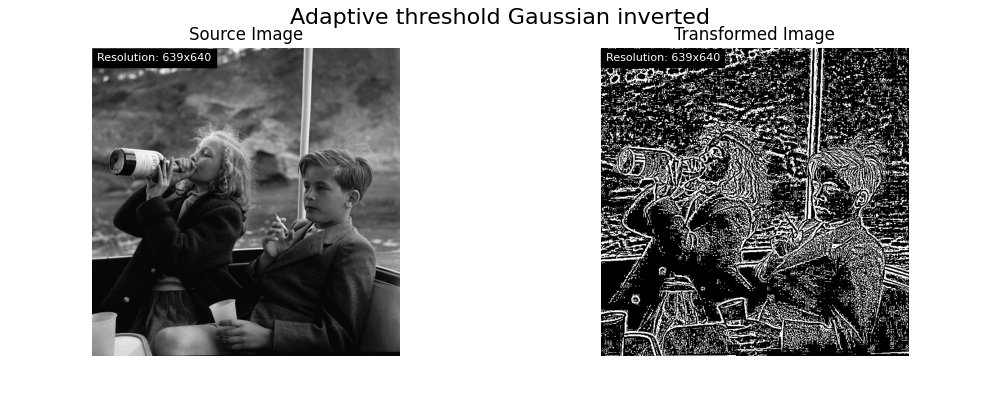
\includegraphics[width=\textwidth]{../results/Adaptive threshold Gaussian inverted.png}
    \caption{Результат адаптивной бинаризации на основе функции Гаусса (инвертированная)}
    \label{img:adaptive_gaussian_inv}
\end{figure}

Данный способ бинаризации очень схож с прошлым, на основе среднего. Однако, он более гладкий и мягкий.


\FloatBarrier

\section{Сегментация изображений}

\subsection{На основе принципа Вебера}

Принцип Вебера подразумевает, что человеческий глаз плохо воспринимает разницу 
уровней серого между $I(n)$ и $I(n) + W(I(n))$, где $W(I(n))$ -- функция Вебера, 
$n$ -- номер класса, $I$ -- кусочно-нелинейная функция градации серого. 

Функция Вебера определяется следующим образом:
\begin{equation}
    W(I) = \begin{cases}
        20 - \frac{12I}{88}, & 0 \le I \le 88, \\
        0.002 (I - 88)^2, & 88 < I \le 138, \\
        \frac{7(I - 138)}{117} + 13.138, & 138 < I \le 255.
    \end{cases}
    \label{eq:weber}
\end{equation}

Можно объединить уровни серого из диапазона $I(n), I(n) + W(I(n))$ затем заменив их один значением интенсивности. 

Алгоритм сегментации состоит из следующих шагов:
\begin{enumerate}
    \item Инициализация начальных условий: номер первого класса $n = 1$, уровень серого $I(n) = 0$. 
    \item Вычисление $W(I(n))$ по формуле \eqref{eq:weber} и присвоение значения интенсивности $I(n)$ всем пикселям из диапазона $I(n), I(n) + W(I(n))$.
    \item Поиск пикселей с интенсивностью выше $G = I(n) + W(I(n)) + 1$. Если найдены, то увеличение номера класса $n = n + 1$. В противном случае закончить работу. 
\end{enumerate}

В результате изображение будет сегментировано на $n$ классов интенсивностью $W(I(n))$. 

Результат применения алгоритма сегментации на основе принципа Вебера к исходному изображению \ref{img:source} представлен на рисунке \ref{img:weber_segmentation}.

\begin{figure}[ht!]
    \centering
    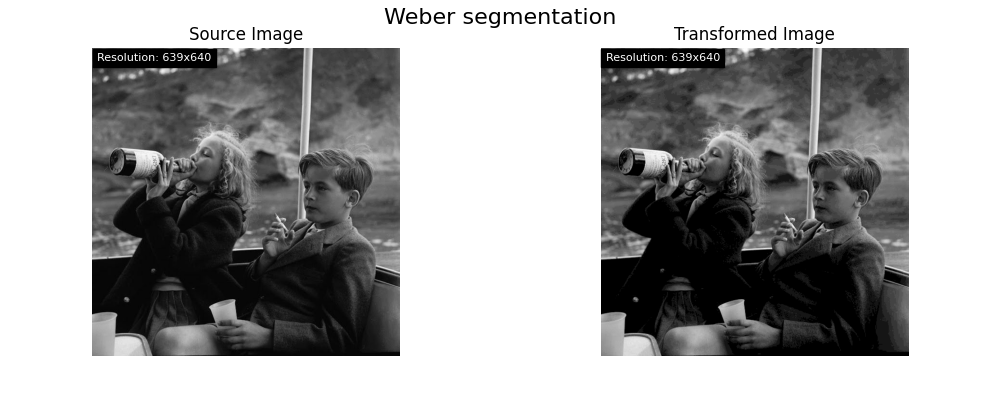
\includegraphics[width=\textwidth]{../results/Weber segmentation.png}
    \caption{Результат сегментации изображения на основе принципа Вебера}
    \label{img:weber_segmentation}
\end{figure}

Визуально не заметно никакой разницы между изображениями. Мы сами сначала даже не поверили, 
что алгоритм работает, но потом сели и честно посчитали каждый пиксель на изображении. 
Цветов оказалось всего 74, ровно как и сказал алгоритм! Вся команда была просто в школе, когда увидела это! 
Вебер красавчик, ставим лайк. 

\subsection{На основе цветового пространства CIE Lab}

В пространстве CIE Lab цветовая информация разделяется на яркость (L) и два цветовых канала (a и b).
Идея алгоритма состоит в разделении изображения на кластеры по цветовому пространству.

\subsubsection{Алгоритм K-means}

Идея алгоритма в определении центров для $k$ кластеров и отнесения каждого пикселя к ближайшему кластеру.

Рассмотрим исходное цветное изображение, которое му будем сегментировать (см. рисунок \ref{img:source_color}).

\begin{figure}[ht!]
    \centering
    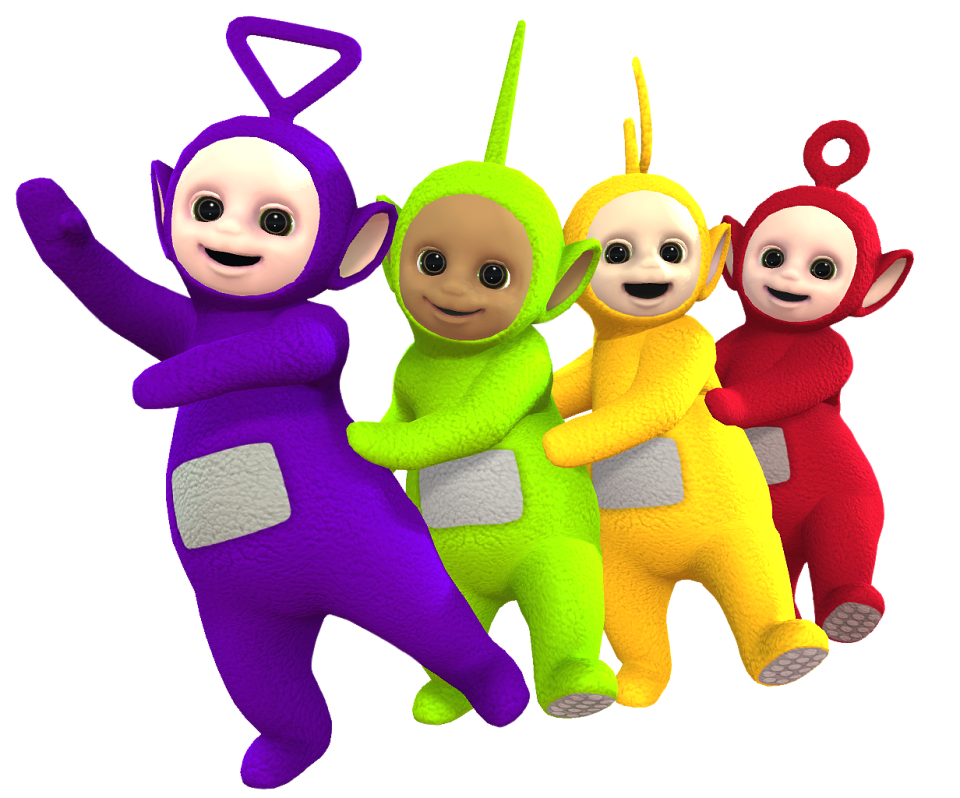
\includegraphics[width=0.8\textwidth]{../puziki.png}
    \caption{Исходное цветное изображение}
    \label{img:source_color}
\end{figure}

Тут у многих возникнут флешбеки из детства, не пугайтесь, дальше будет хуже. 

После применения алгоритма для нахождения 5 кластеров получим результат, представленный на рисунке \ref{img:kmeans_segmentation}.
\begin{figure}[ht!]
    \centering
    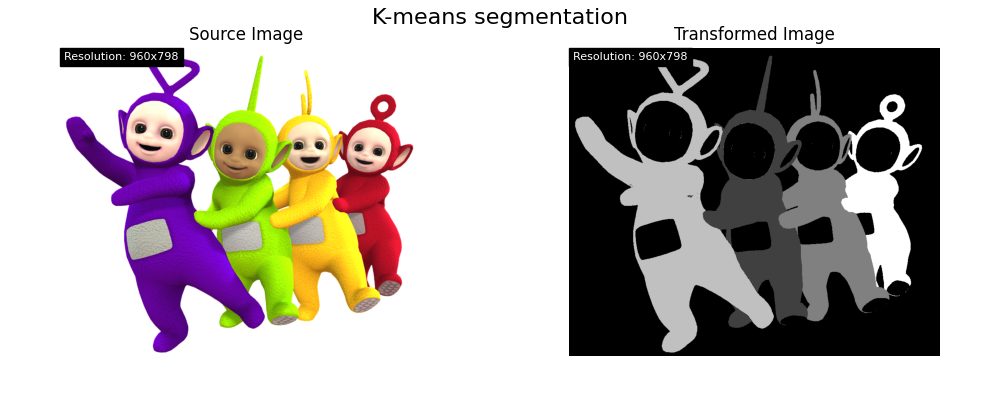
\includegraphics[width=\textwidth]{../results/K-means segmentation.png}
    \caption{Результат сегментации изображения с использованием алгоритма K-means}
    \label{img:kmeans_segmentation}
\end{figure}
Разные оттенки серого -- это разные кластеры. 

Теперь рассмотрим каждый из кластеров отдельно: 

\begin{figure}[ht!]
    \centering
    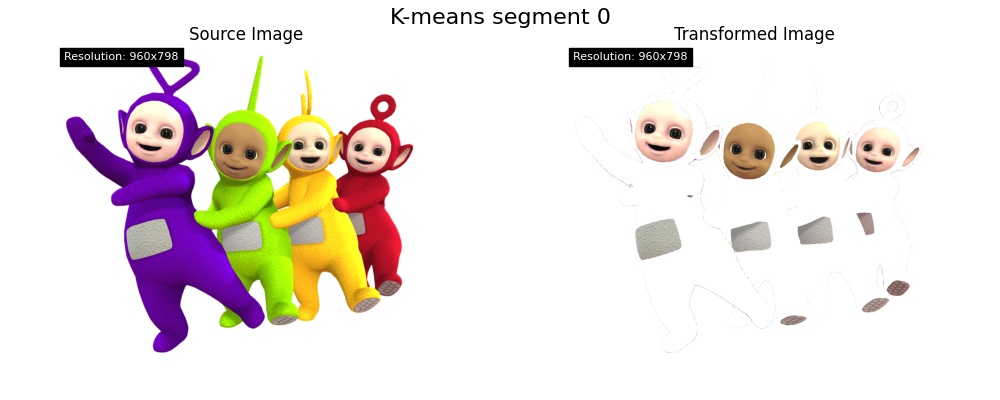
\includegraphics[width=\textwidth]{../results/K-means segment 0.png}
    \caption{Кластер 0}
    \label{img:kmeans_cluster_0}
\end{figure}

\begin{figure}[ht!]
    \centering
    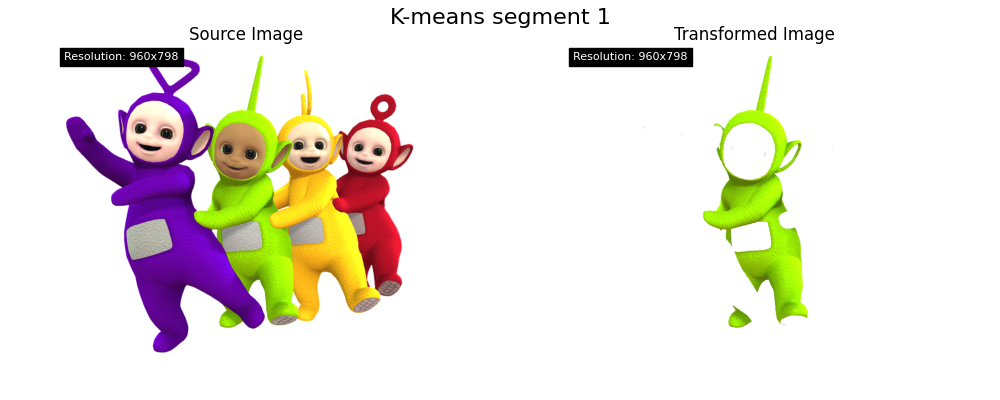
\includegraphics[width=\textwidth]{../results/K-means segment 1.png}
    \caption{Кластер 1}
    \label{img:kmeans_cluster_1}
\end{figure}

\begin{figure}[ht!]
    \centering
    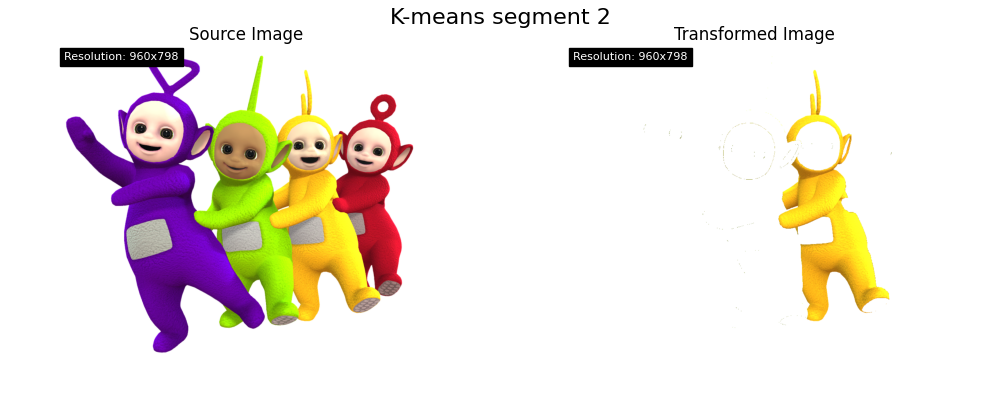
\includegraphics[width=\textwidth]{../results/K-means segment 2.png}
    \caption{Кластер 2}
    \label{img:kmeans_cluster_2}
\end{figure}

\begin{figure}[ht!]
    \centering
    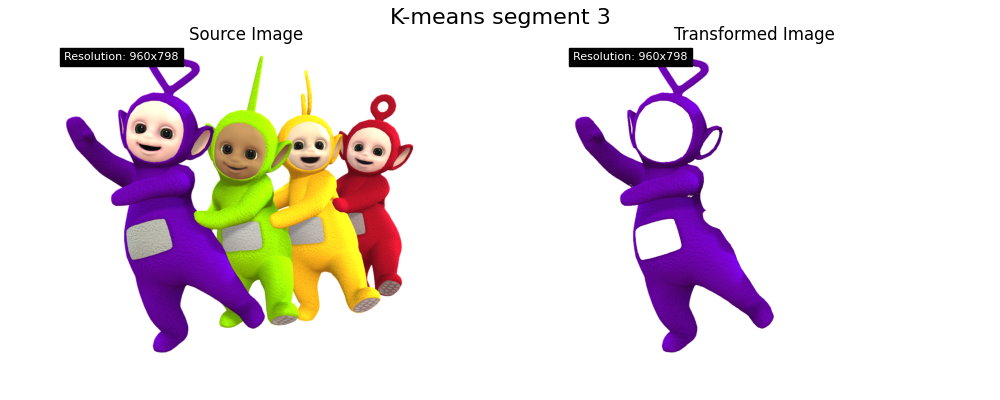
\includegraphics[width=\textwidth]{../results/K-means segment 3.png}
    \caption{Кластер 3}
    \label{img:kmeans_cluster_3}
\end{figure}

\begin{figure}[ht!]
    \centering
    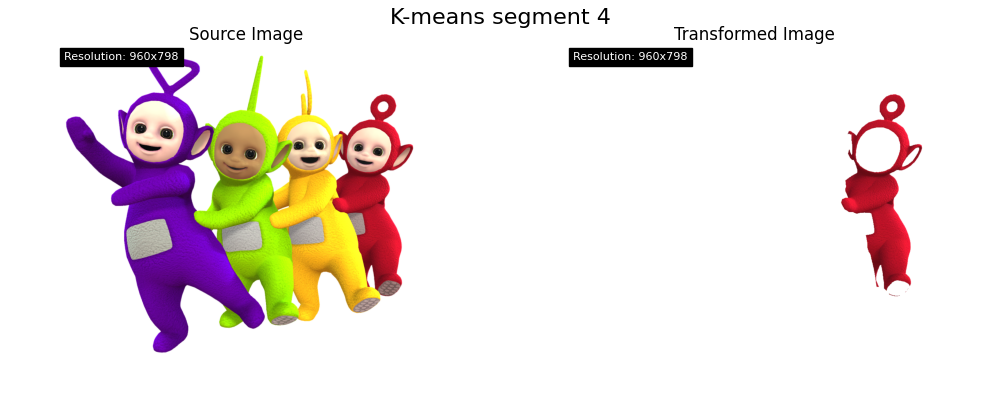
\includegraphics[width=\textwidth]{../results/K-means segment 4.png}
    \caption{Кластер 4}
    \label{img:kmeans_cluster_4}
\end{figure}

\FloatBarrier
Видно, что на каждом кластере, как и ожидалось, преобладает один цвет. Телепузиков удалось разделить друг от друга. 

Теперь можно заменить $a, b$ составляющие каждого пикселя на среднее значение по кластеру, перейти обратно в пространство RGB и получить сегментированное изображение (см. рисунок \ref{img:kmeans_segmentation_RGB}).

\begin{figure}[ht!]
    \centering
    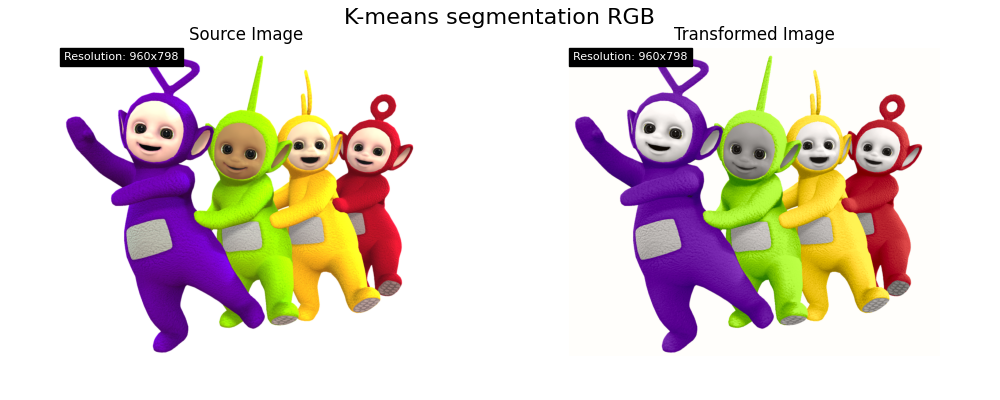
\includegraphics[width=\textwidth]{../results/K-means segmentation RGB.png}
    \caption{Сегментированное изображение с использованием алгоритма K-means}
    \label{img:kmeans_segmentation_RGB}
\end{figure}
При этом яркостная составляющая изображения остается неизменной, что позволяет сохранить детали изображения.

\FloatBarrier
\subsection{Текстурная сегментация}

В работе используется статистический подход, который описывает текстуру сегмента 
как гладкую, грубую или зернистую. 

Исходное изображение, содержащее два различных текстурных участка, представлено на рисунке \ref{img:texture_source}.

\begin{figure}[ht!]
    \centering
    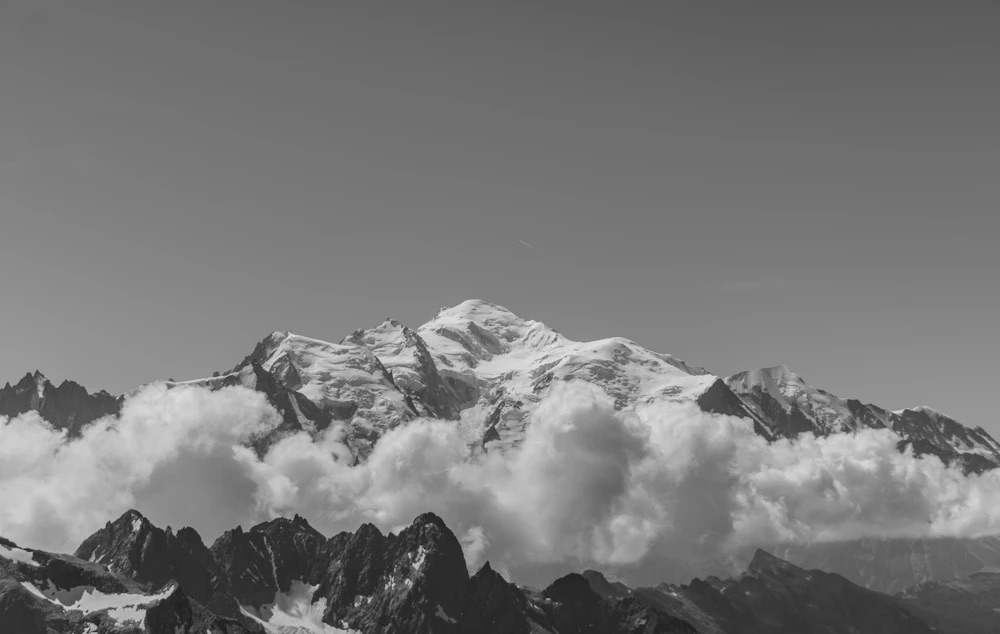
\includegraphics[width=\textwidth]{../mountain.jpeg}
    \caption{Исходное изображение для текстурной сегментации}
    \label{img:texture_source}
\end{figure}

Будем рассматривать интенсивность изображения $I$ как случайную величину $z$, которой соответствует вероятность распределения 
$p(z)$, вычисляемая из гистограммы изображения. \textit{Центральным моментом} порядка $n$
случайной величины $z$ называется параметр $\mu_n(z)$, вычисляемый по формуле: 
\begin{equation}
    \mu_n(z) = \sum_{i = 0}^{L - 1} (z_i - m)^n p(z_i)
    \label{eq:mu_n}
\end{equation}
где $L$ -- количество уровней интенсивности, $m$ -- среднее значение случайной величины $z$: 
\begin{equation}
    m = \sum_{i = 0}^{L - 1} z_i p(z_i)
\end{equation}
Из \eqref{eq:mu_n} следует, что $\mu_0 = 1$ и $\mu_1 = 0$. 

Для описания текстуры изображения важна \textit{дисперсия случайной величины}, равная второму моменту 
$\sigma^2(z) = \mu_2(z)$ и являющаяся мерой яркостного контраста, которую можно использовать для вычисления 
признаков \textit{гладкости}. Введем меру относительной гладкости $R$:
\begin{equation}
    R = 1 - \frac{1}{1 + \sigma^2(z)}
\end{equation}
которая равна нулю для областей с постоянной интенсивностью (нулевой дисперсией) и приближающаяся к единице 
для больших значений дисперсии $\sigma^2(z)$. Для полутоновых изображений с интервалом интенсивности $[0, 255]$ 
необходимо нормировать дисперсию до интервала $[0, 1]$. Нормирование осуществляется делением дисперсии $\sigma^2(z)$
на $(L - 1)^2$. В качестве характеристики текстуры часто используется \textit{стандартное отклонение}:
\begin{equation}
    s = \sigma(z)
\end{equation}
Третий момент является \textit{характеристикой симметрии гистограммы}. 

Для оценки текстурных особенностей используется 
функция \textit{энтропии} $E$, определяющая разброс интенсивностей соседних пикселей. 
\begin{equation}
    E = -\sum_{i = 0}^{L - 1} p(z) \log_2 p(z_i)
\end{equation}

Еще одной важной характеристикой, описывающей текстуру, является \textit{мера однородности} $U$, оценивающая равномерность гистограммы: 
\begin{equation}
    U = \sum_{i = 0}^{L - 1} p^2(z_i)
\end{equation}
После вычисления какого-либо признака или набора признаков необходимо построить бинарную маску, на основе которой и будет проводиться сегментация. 

Энтропия исходного изображения в окрестности $(9 \times 9)$ каждого пикселя и ее бинаризованной мо методу Отсу вариант представлены на рисунках \ref{img:texture_entropy} и \ref{img:texture_entropy_bin} соответственно.
\begin{figure}[ht!]
    \centering
    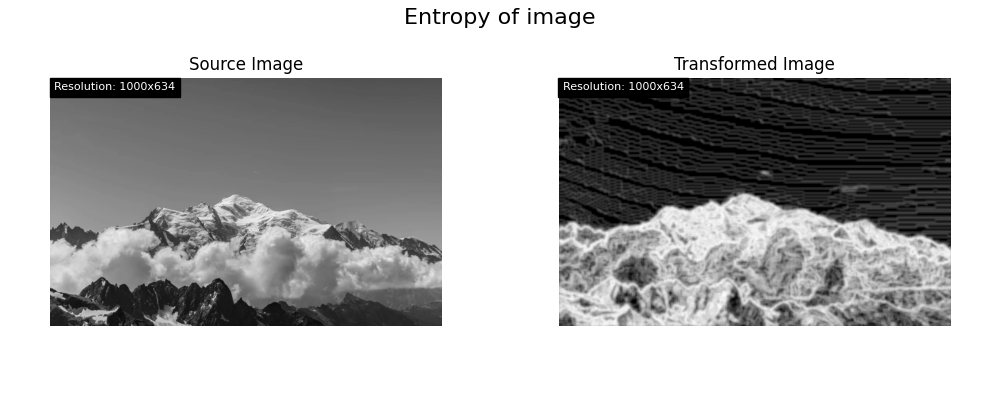
\includegraphics[width=\textwidth]{../results/Entropy of image.png}
    \caption{Энтропия исходного изображения}
    \label{img:texture_entropy}
\end{figure}

\begin{figure}[ht!]
    \centering
    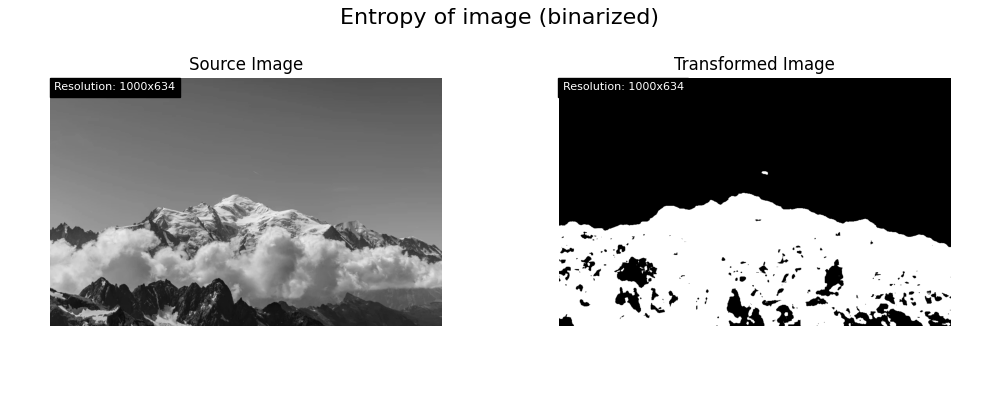
\includegraphics[width=\textwidth]{../results/Entropy of image (binarized).png}
    \caption{Бинаризованная энтропия изображения}
    \label{img:texture_entropy_bin}
\end{figure}

\FloatBarrier
После этого необходимо использовать морфологические фильтры для того, чтобы удалить связные области, содержащее
менее заданного количества пикселей, а затем для удаления внутренних дефектов формы. (см. рисунок \ref{img:BW_E_SR} и \ref{ing:BW_E_SR_OR}).

\begin{figure}[ht!]
    \centering
    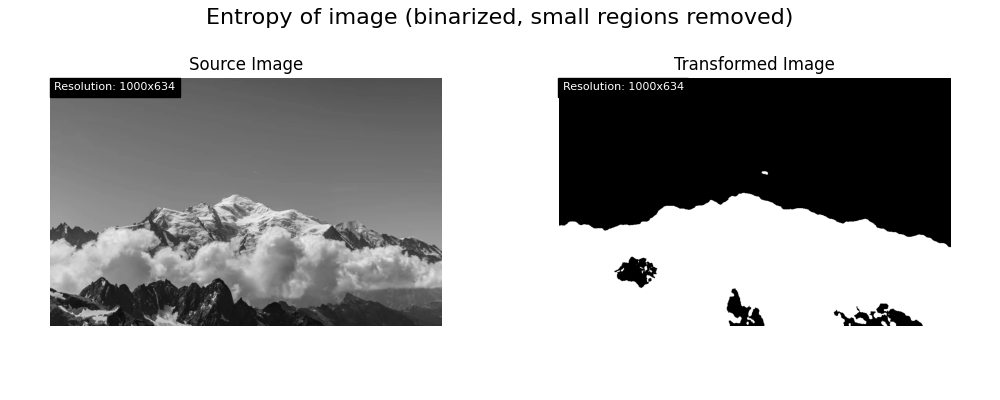
\includegraphics[width=\textwidth]{../results/Entropy of image (binarized, small regions removed).png}
    \caption{Бинаризованная энтропия изображения после удаления малых областей}
    \label{img:BW_E_SR}
\end{figure}

\begin{figure}[ht!]
    \centering
    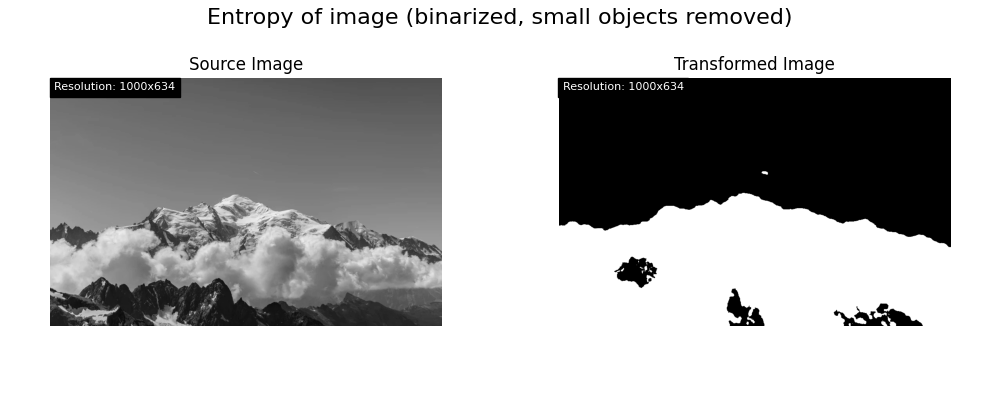
\includegraphics[width=\textwidth]{../results/Entropy of image (binarized, small objects removed).png}
    \caption{Бинаризованная энтропия изображения после удаления малых областей и внутренних дефектов}
    \label{ing:BW_E_SR_OR}
\end{figure}

Изображение с нанесенными контурами после сегментации представлено на рисунке \ref{img:regions}.
Видим, что текстуры на изображении разделены на разные области корректно. 

\begin{figure}[ht!]
    \centering
    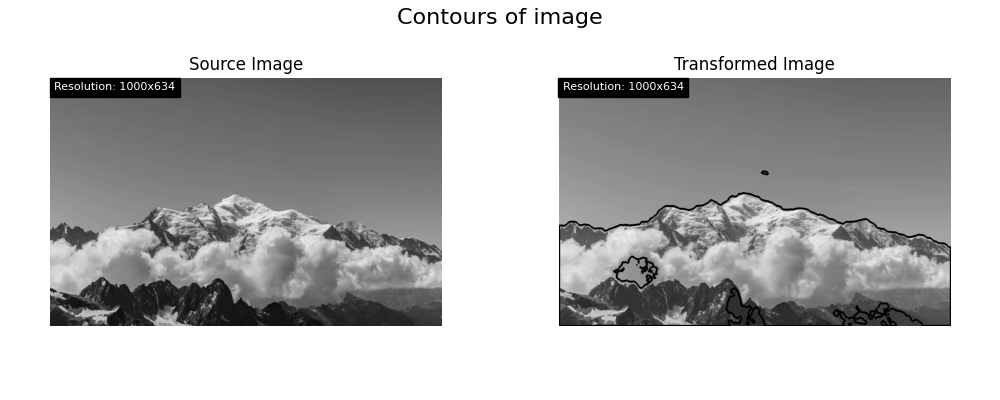
\includegraphics[width=\textwidth]{../results/Contours of image.png}
    \caption{Изображение с контурами после сегментации}
    \label{img:regions}
\end{figure}

Отдельно можно посмотреть на \textit{гладкие} и \textit{грубые} области изображения (см. рисунки \ref{img:smooth} и \ref{img:rough}).

\begin{figure}[ht!]
    \centering
    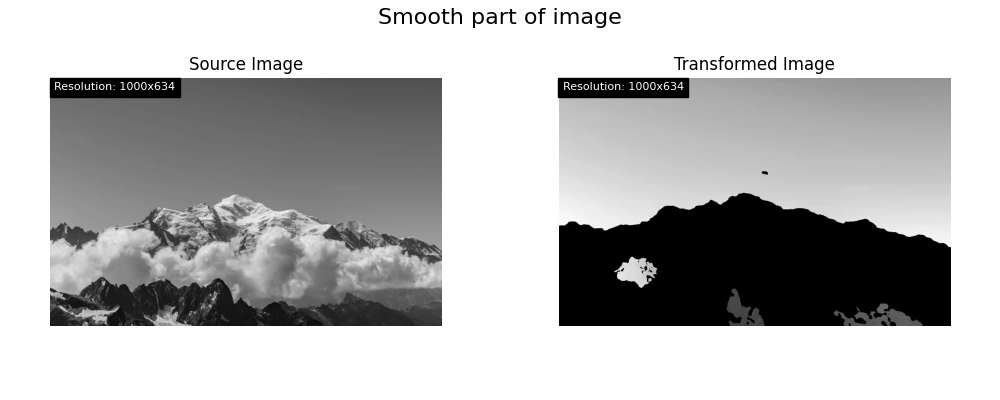
\includegraphics[width=\textwidth]{../results/Smooth part of image.png}
    \caption{Гладкие области изображения}
    \label{img:smooth}
\end{figure}

\begin{figure}[ht!]
    \centering
    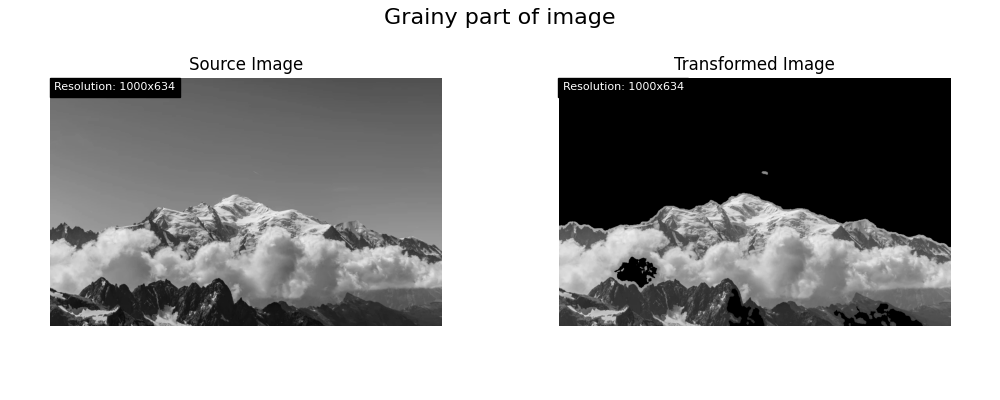
\includegraphics[width=\textwidth]{../results/Grainy part of image.png}
    \caption{Грубые области изображения}
    \label{img:rough}
\end{figure}

\begin{table}[ht!]
    \centering
    \begin{tabular}{|c|c|c|c|c|c|c|}
        \hline
        Область & $m$ & $\mu_3(z)$ & $R$ & $\sigma$ & $E$ & $U$ \\
        \hline
        Гладкая &  116.7 & 0 & 0.0045 & 0.0674 & 5.6305 & 0.0249\\
        \hline
        Все изображение & 120.2 & -0.0004 &  0.0182 & 0.1363 & 6.8281 & 0.0125 \\
        \hline
        Грубая &  125.1 & -0.0379 & 0.0012 & 0.1948 & 7.4204 & 0.0061\\
        \hline
    \end{tabular}
    \caption{Параметры текстурных областей}
    \label{tab:texture_params}
\end{table}

\FloatBarrier
В таблице \ref{tab:texture_params} видим, что при уменьшении \textit{гладкости} области, для которой определялись параметры: 
\begin{itemize}
    \item Значение \textbf{гладкости} $R$ \textbf{уменьшается}
    \item Значение \textbf{меры однородности} $U$ \textbf{уменьшается}
    \item Значение \textbf{стандартного отклонения} $\sigma$ \textbf{увеличивается}
    \item Значение \textbf{энтропии} $E$ \textbf{увеличивается}
\end{itemize}

Есть закономерность значений параметров от текстуры области, для которой они находились. 
Таким образом, можно сделать вывод, что параметры текстурных областей могут быть использованы для сегментации изображений 
и определения \textit{гладкости} текстурных областей.




\section{Выводы}

В результате работы нам удалось изучить методы сегментации и бинаризации изображений. 

Мы рассмотрели алгоритмы бинаризации по среднему значению, по модулю градиента, 
по метода Отсу, адаптивную бинаризацию, а также сегментацию по принципу Вебера.

Кроме того, был рассмотрен алгоритм текстурной сегментации изображений. 
Нам удалось выделить мягкие и грубые текстуры на изображении, сегментировать его по этому принципу. 

Была рассмотрена работа с цветовым пространством CIE Lab, сегментация изображений по цвету в этом пространстве.

А вообще, мы молодцы. Как и обещали, отчет был отправлен на подпись к Путину. 


\section{Ответы на вопросы}

\newcounter{question}
\setcounter{question}{0}

\newcommand{\question}[1]{\item[Q\refstepcounter{question}\thequestion.] #1}
\newcommand{\answer}[1]{\item[A\thequestion.] #1}


\begin{itemize}

    \question{В каких случаях целесообразно использовать сегментацию по принципу Вебера?}
    \answer{Для уменьшения количества цветов в полутоновом изображении без потери качества. 
    
    Может быть использовано как метод сжатия изображений, как предварительная подготовка изображения перед другими методами обработки.}
    
    \question{Какие значения имеют цветовые координаты a и b цветового пространства CIE Lab в полутновом изображении?}
    \answer{Цветовые координаты $a$ и $b$ цветового пространства CIE Lab в полутоновом изображении могут принимать значения 
    от $-128$ до $127$. Координата $a$ отвечает за положение цвета от зеленого до красного, а координата $b$ отвечает за положение цвета от синего до желтого.} 

    \question{Зачем производить сегментацию в цветовом пространстве CIE Lab, а не в исходном RGB}
    \answer{В этом цветовом пространстве яркость цвета хранится отдельно, что позволяет не учитывать ее влияние при сегментации.
    
    Более того, в CIE Lab расстояние между точками в цветовом пространстве более равномерно, чем в RGB. Это облегчает сегментацию и классификацию цветов. }

    \question{Что такое цветовое пространство и цветовой охват?}
    \answer{Цветовое пространство — это абстрактная модель, которая описывает, как цвета представлены и интерпретируются в компьютерных системах, фотографии, видео и других медиа. Оно определяет, какие цвета можно отобразить или кодировать в конкретной системе, что и является цветовым охватом.}
\end{itemize}
    
\FloatBarrier
\begin{figure}
    \centering
    
\includegraphics[width=0.5\textwidth]{./media/sig.jpg}
    \caption{Подпись Путина}
    \label{img:putin_signature}
\end{figure}
 % Content

\end{document}